\documentclass[10pt]{article}
\usepackage{mathtools}
\usepackage{amssymb}
\usepackage{enumitem}
\usepackage[left=1.5cm, right=2cm, top=1cm, bottom=2cm]{geometry}
\usepackage{tikz}
\usepackage{graphicx}
\graphicspath{ {./images/} }
\usetikzlibrary{arrows,shapes,automata,petri,positioning,calc}
\setlength\parindent{0pt}
\title{Agile Recap - Answers/Summary}
\date{}
\author{}
\newcommand*\circled[1]{\tikz[baseline=(char.base)]{
            \node[shape=circle,draw,inner sep=2pt] (char) {#1};}}
\newcommand{\caselist}[1]{\begin{enumerate}[label=\protect\circled{C\arabic*}]#1\end{enumerate}}
\newcommand*{\true}{\circled{V}}
\newcommand*{\false}{\circled{F}}
\newcommand\xeq[1]{\,\stackrel{\mathclap{\normalfont\mbox{\tiny{#1}}}}{=}\,}

\begin{document}
\maketitle
If stuck, reduce functionality and keep to the schedule, instead of trying to modify the schedule or add developers
\begin{itemize}
\item '9 pregnant women don't make a baby in a month'. Essentially, adding more developers rarely speeds up development in the short-term (can work long-term, but not relevant to this question)
\item K eeping to deadlines in timeboxed iterations/sprints ensures a predictable delivery cycle and workload
\item Lengthening development cycles reduces feedback from deliveries
\item Reprioritization helps deliver on critical features while allowing those that appear less essential to be deferred
\item Sustainable pace (No death marches or whatever)
\end{itemize}
Big upfront requirements, why Agile opposes them and why some are still beneficial
\begin{itemize}
\item Agile seeks adaptability, feedback, delivering value early
\begin{itemize}
\item Collecting big upfront requirements delays the start of development
\item Predefined requirements/product specifications hinder adaptability \& customer feedback
\item Embrace change
\item Working software over comprehensive documentation
\item Incremental + iterative approach
\item Reduce risk + waste
\end{itemize}
\item Some upfront planning is useful
\begin{itemize}
\item Define a product vision + goals, tech stack, etc. (As we did in Sprint 0)
\item Set architectural foundations. Concerns over scalability, security, and integration should be considered early on in a project
\item External dependencies, risk analysis, legal requirements, budgeting, stakeholders cannot be 'discovered iteratively'
\end{itemize}
\end{itemize}
Thinking on the video of the ping pong ball, establish a flow before optimizing resources.\\
Importance of having customer relations
\begin{itemize}
\item XP has a customer representative role within teams (This isn't very viable, but still you get the point)
\item Agile teams should have some role that interfaces with customers.
\item Not all customer feedback is great - Customers don't really know what they want much of the time
\end{itemize}
Kano model:\\
Graph satisfaction on y-axis, level of fulfillment on x-axis.\\
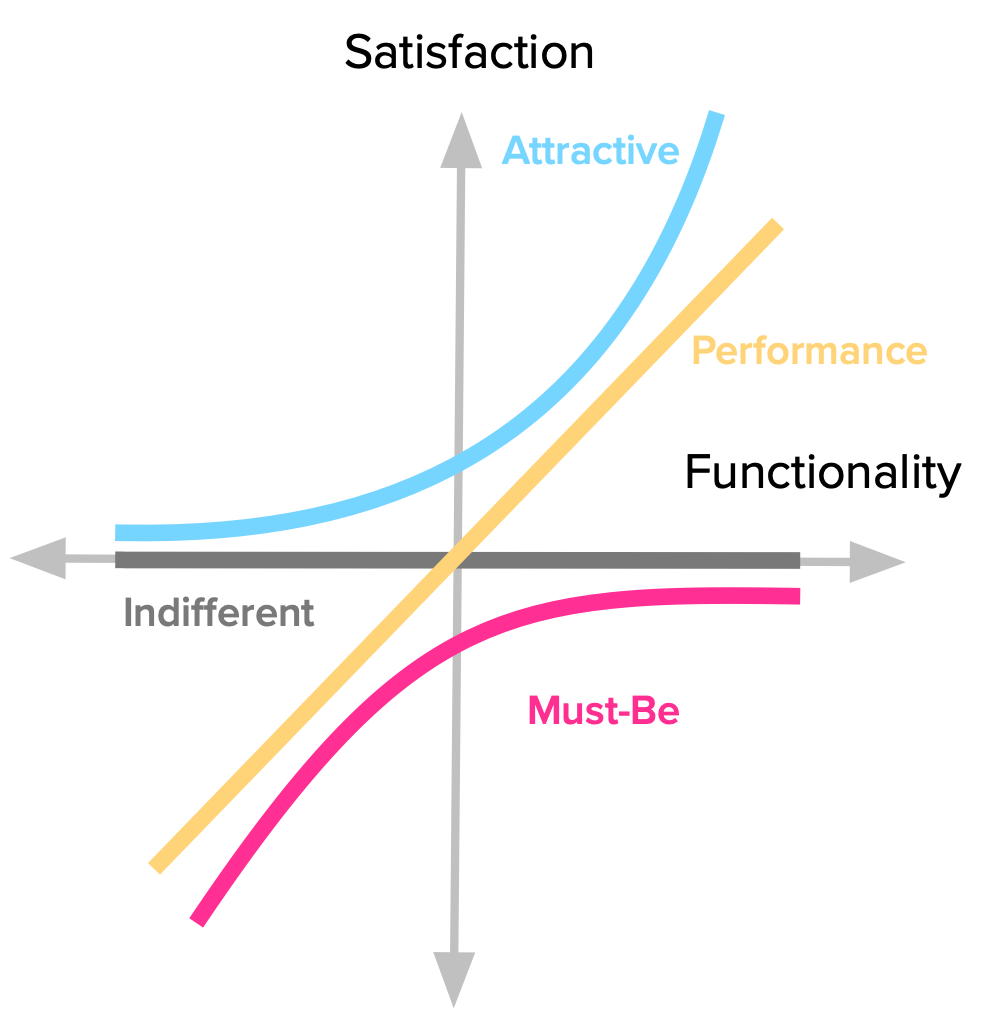
\includegraphics[width=5cm, height=5cm]{kano}\\
Projects/developers should be executed at a sustainable pace, sprints should be planned with cushions of leftover time for the team members in case of unforeseen obstacles\\
Additive vs Multiplicative complexity
\begin{itemize}
\item Additive complexity refers to the linear growth of software complexity that simply results from the growth of a codebase/product
\item Multiplicative complexity is often the result of a poorly designed architecture; increasing dependencies make it such that every additional feature multiplies the number of interactions, increasing complexity further
\end{itemize}
Accepting vs liking change
\begin{itemize}
\item I wouldn't dwell too much on this, the concept is self-explanatory
\item PMs don't really enjoy change, but as part of Agile teams they should be willing to expect and accept it
\end{itemize}
Weighted-shortest-job-first feature prioritization
\begin{itemize}
\item I vaguely remember there being a slide and a short exercise on this, there will be an exam question about it, I will probably not have read the slide because I don't wanna search for it, assuming the concept is self-explanatory and then realize I probably should have at least skimmed the slide.
\end{itemize}
Iterative development
\begin{itemize}
\item Small incremental improvements. Break work down into iterations (Sprints in Scrum), each should produce a shippable product increment. Deliver working software in small steps rather than delivering all at once
\item Frequent feedback and adaptation. Sprint review, demos, user testing are some of the feedback loops involved in iterations.
\item Continuous learning \& improvement. Retrospectives and learning on each cycle improve processes and decision-making
\item Value prioritization. Features are delivered based on business value, backlog is refined to reflect changing priorities
\item Reduced risk \& early problem detection
\end{itemize}
\begin{itemize}
\item In Scrum, iterations are defined as sprints (1-4 weeks) where a set of backlog items are developed and reviewed
\item In Kanban, Continuous iteration occurs through small batch delivery and WIP limits
\item In XP, there are frequent releases (sometimes multiple per day) with constant refactoring and feedback
\end{itemize}
Requirements vs Scenarios
\begin{itemize}
\item Requirements cover the complete scope of functionalities, user stories cannot replace these, as you can't fully define a specification with them
\item Sometimes requirements are necessary, think of legal requirements, architectural, performance, etc.
\end{itemize}
Scrum ceremonies
\begin{itemize}
\item Daily meeting
\item Sprint demo
\item Sprint planning
\begin{itemize}
\item Planning Poker
\end{itemize}
\end{itemize}
Shared code ownership \& cross-functional teams
\begin{itemize}
\item In shared code ownership, the entire team is responsible for all code, instead of having individual devs responsible for/'owning' sections
\item Cross-functional teams refers to teams with knowledge from different areas. The professor speaks of wanting 'T-shaped' team members in Volvo Cars, with expertise in one specific area but at least surface-level knowledge on the rest of the areas relevant to the project
\end{itemize}
\begin{itemize}
\item Shared code ownership can improve code quality by bringing more eyes to each piece of code, speed up development by reducing bottlenecks on specific devs, encourages knowledge sharing and makes refactoring easier (no approval from a specific dev)
\item Inconsistent coding styles, merge conflicts \& overwrites, reduced sense of ownership/accountability and a need for strong communication are some drawbacks of shared code ownership
\item Cross-functional teams can speed up delivery by reducing handoffs between teams, they improve collaboration and flexibility and are able to consider more aspects of a product, improving quality
\item Cross-functional teams can face challenges with coordination, conflicting priorities, skill gaps and scaling (managing cross-functional teams in large organizations is complex)
\end{itemize}
Personal thoughts on pair programming
\begin{itemize}
\item IDK, form some and write them on here
\item XP likes it
\end{itemize}
Test-Driven Development - Know 5 steps in detail, be able to provide examples (our own work is relevant, mention the Unit tests we wrote with JUnit for our backend, be aware that we wrote those tests after implementing the feature though so maybe google a better example and write it down here please uwu)
\begin{enumerate}
\item Quickly add a test
\item Run all tests, see the new one fail
\item Make a small change
\item Run all tests again, see them succeed
\item Refactor \& remove duplication
\end{enumerate}
Extreme Programming (XP)\\
Practices - Please list them down here if you have the slide with them on you :D. We need to be able to explain them listing them by heart is not necessary though\\
I am starting to believe that this subject is not worth the 3 credits I'll be getting at my home uni\\
Also, someone tell the student representatives that is the professor wants to forego the exam but also ensure that we actually learn the contents while keeping the primary focus on the project then having us answer the questions to the exam by sections as group assignments throughout the project would be a very effective way of achieving this while also being much less of a pain in the big O for all of us.
\begin{itemize}
\item Here is where I would list some XP practices and their definitions, if I had any
\end{itemize}
Product Owner, Scrum Master, Dev Team roles
\begin{itemize}
\item 
\end{itemize}
Product backlog, why it should be detailed, what a DEEP backlog is, why we want ONE product backlog\\
Difference between project and product\\
User stories, INVEST format\\
Be able to break down a functionality into around 10 user stories:\\
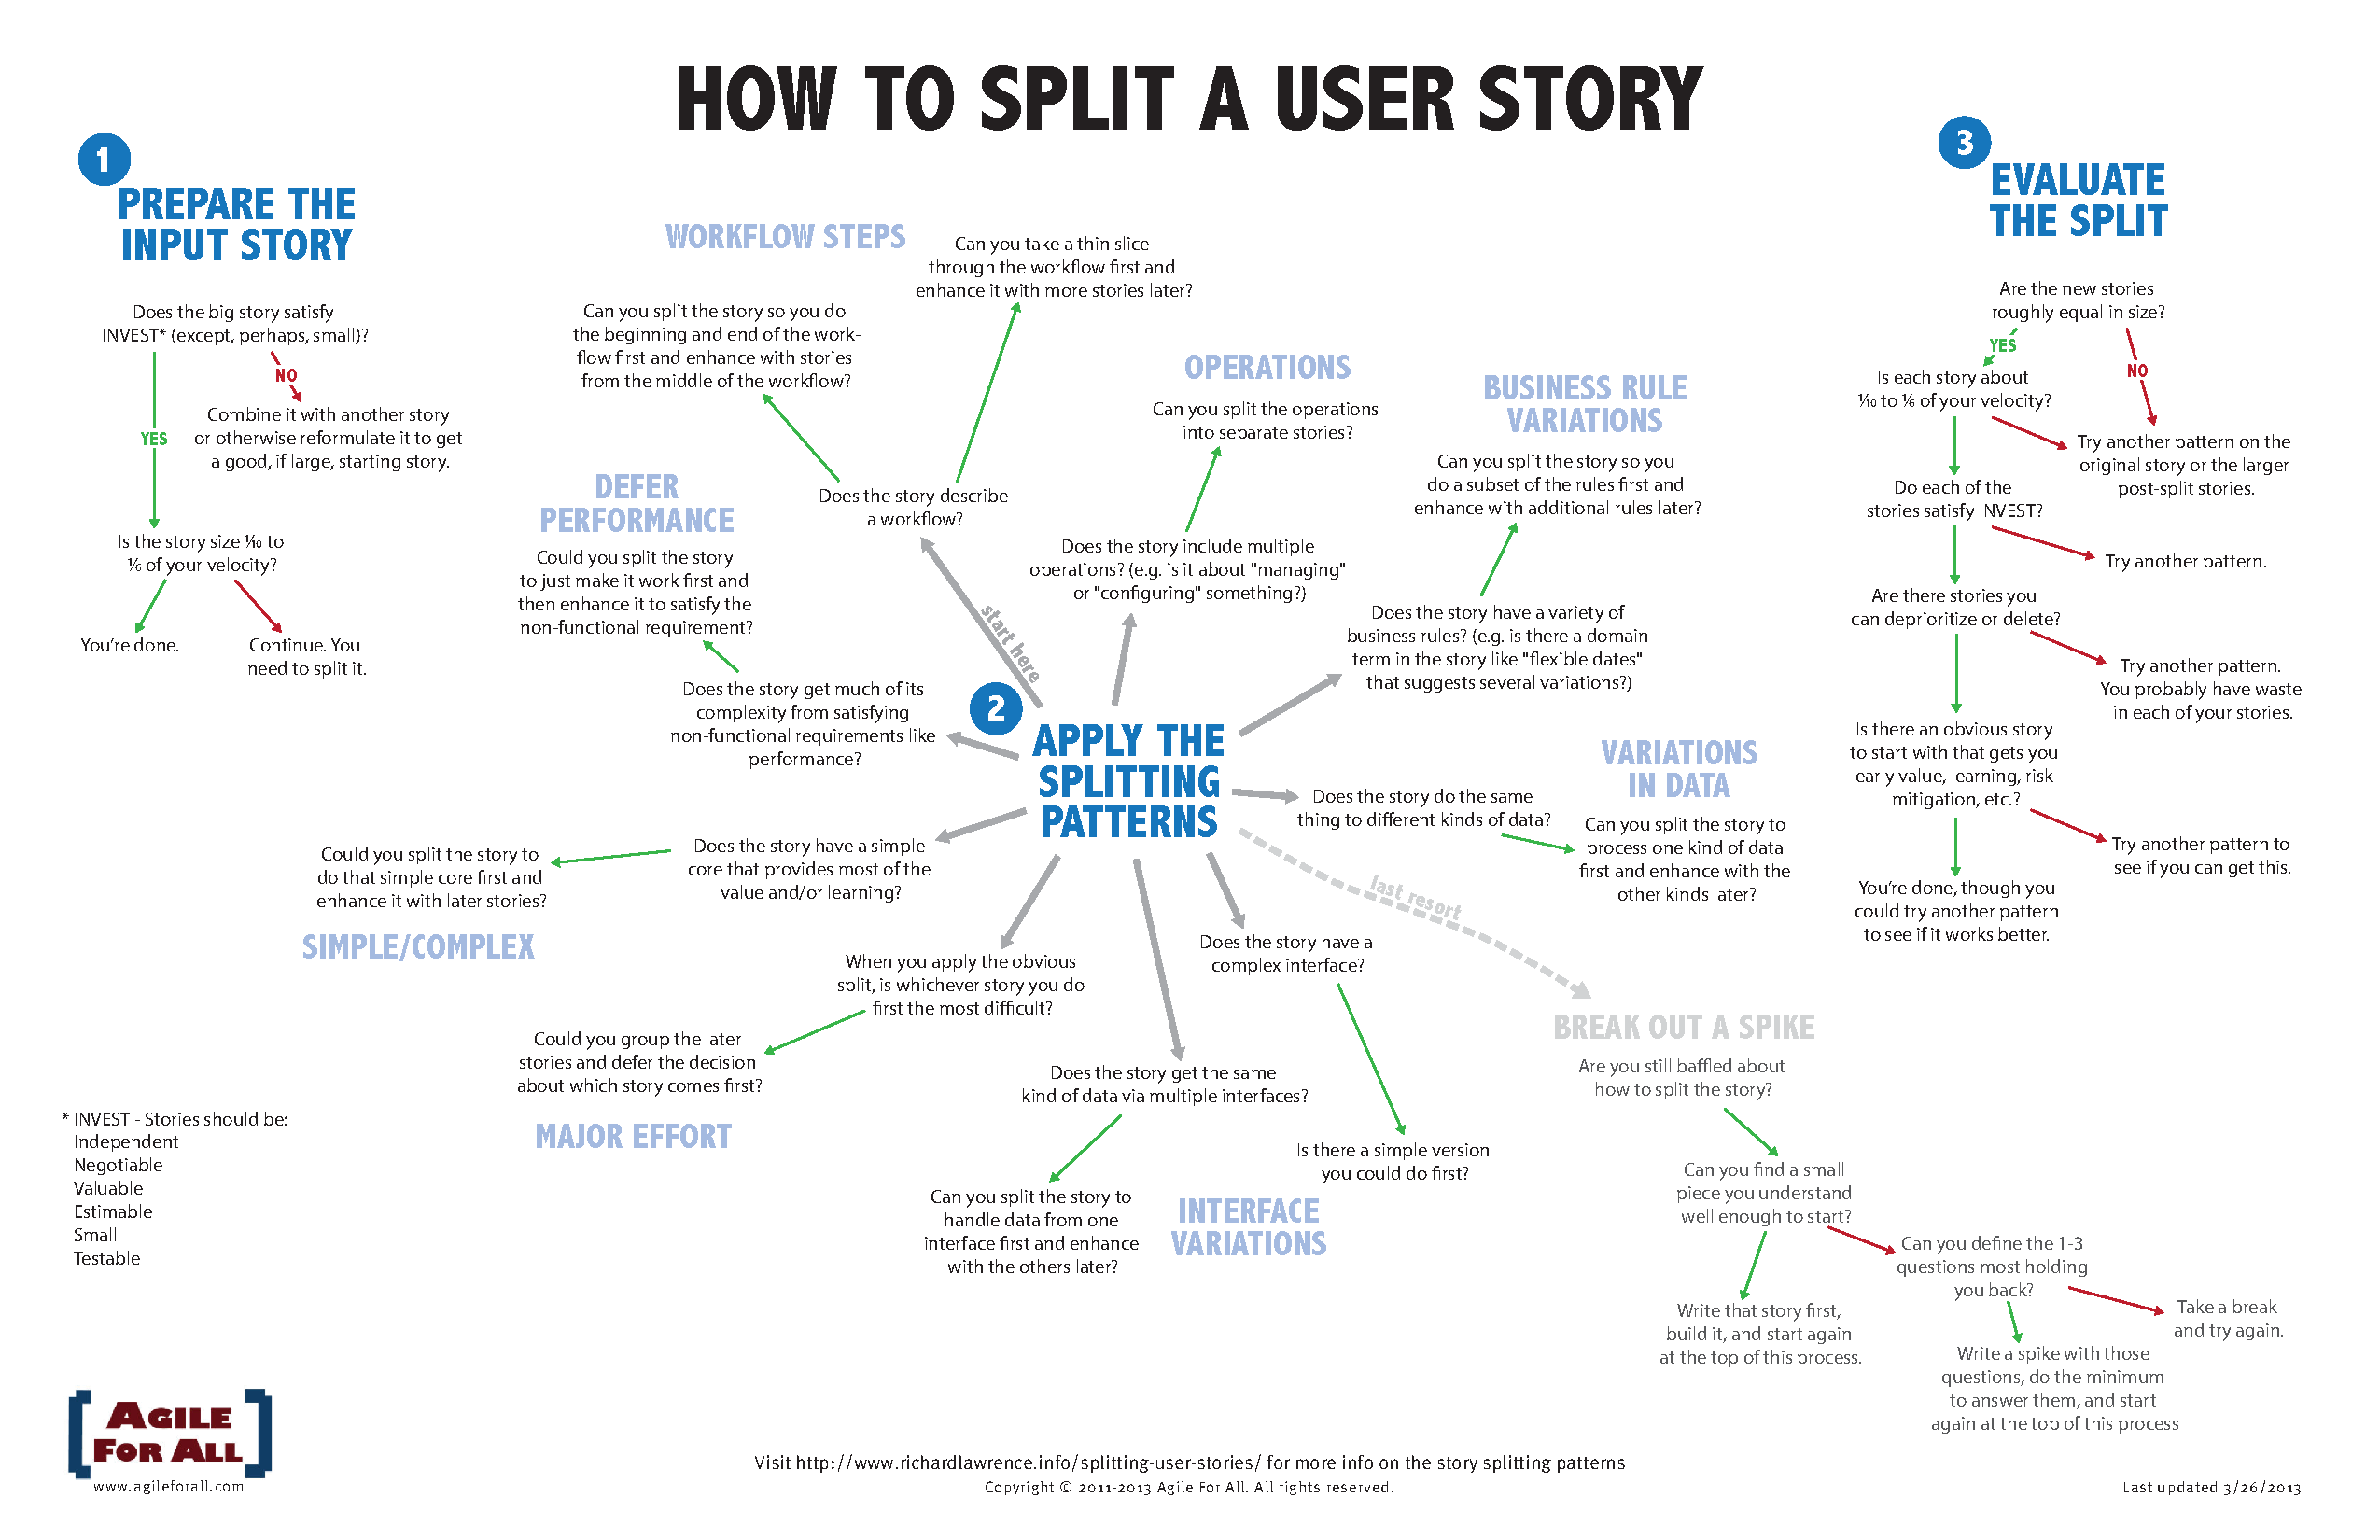
\includegraphics[width=12cm, height=10cm]{userstories-flowchart}\\
Functional vs Non-functional requirements
\begin{itemize}
\item Functional
\item Non-functional
\end{itemize}

\end{document}
